% Chapter 2
\hyphenation{student/teacher}

\chapter{Problem Definition} % Main chapter title
%\epigraph{A fancy quote.}{Me}

\label{current_process} % For referencing the chapter elsewhere, use \ref{Chapter2} 

\lhead{Chapter 2. \emph{Problem Definition}} % This is for the header on each page - perhaps a shortened title

This chapter explains some basic concepts commonly found in the literature. A comprehensive explanation of example constraints and their relative importance is also shown.  
%----------------------------------------------------------------------------------------

\section{Fundamental Concepts}

In order to better understand this work, it is important to define some concepts that may have different meanings in other works and in the literature. 

The following list of concepts is oriented to the Portuguese scenario \citep{bullet_paper} \citep{recent_dev_patat}.  

\begin{itemize}
	\item \textbf{Constraint} - A constraint is a specified rule that must or should be respected. If the constraint is specified as hard, then it must be followed. Soft constraint should be respected as much as possible.  
	\item \textbf{Conflict} - A conflict represents an undesirable situation where two events conflict somehow with each other (e.g., teachers in common at the same time slot) and must not happen.
	\item \textbf{Feasible Timetable} - A timetable is considered feasible when all events are scheduled and no hard constraint is violated.  
	\item \textbf{Course} - An Educational Institution may offer various courses. Each course has a set of curricular plans, usually one for each year of the duration of the course.
	\item \textbf{Curricular Plan} - A curricular plan is a set of subjects or disciplines to be taken by students wishing to obtain a given degree.
	\item \textbf{Subject} - A subject is a discipline taught one or more times a week, under different possible \textbf{typologies} (e.g., theoretical, practical). It is usually taught in a specific part of the year (e.g., annual, half a year, quarterly). Also, the same subject may be taught repeatedly for the different groups of students and is usually called a \textbf{turn} or \textbf{class}.  
	\item \textbf{Class} - A class represents a set of students having the same subject at the same time. This class may then be broken down in a couple of lectures (events) and this set of students remain together throughout the week. It is important to note that the schedules are defined at this level, i.e, this particular class will have a set of lectures scheduled along the week.
	\item \textbf{Group} - A group is a set of students who follow the same curricular plan and share the same timetable.
	\item \textbf{Event} - An event is the basic unit to be scheduled. It represents a lecture that is lectured by a teacher to a group of students, at a given time, with a given duration and occurs in a given classroom. Each event occurs in a set of weeks, representing the duration of the subject and is subject to a set of constraints that should or must be respected. 
	\item \textbf{Time slot} - A time slot is the basic time unit and it is associated to the assigned events. An event may have a duration of several time slots.
\end{itemize}

Figure \ref{fig:portuguese_curr_plan} illustrates some of these concepts.
 	   
\begin{figure}[htbp]
	\centering
		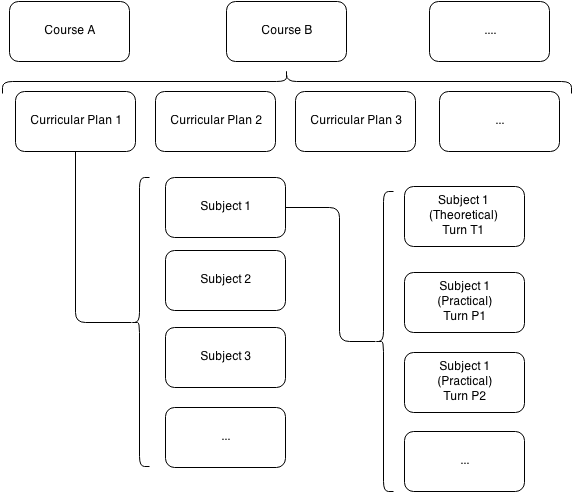
\includegraphics[scale=0.55]{./Figures/curricular_structure.png}
		\rule{35em}{0.5pt}
	\caption[The university curricular structure in Portugal]{The university curricular structure in Portugal}
	\label{fig:portuguese_curr_plan}
\end{figure}

There are many variations of the timetabling problem. When students, teachers and classes are involved, we are usually faced with three main categories \citep{introduction_timetable}, \citep{british_examination_survey}:

\begin{itemize}
	\item Class/Teacher timetabling - The weekly scheduling of lectures. Each lecture is an instance of a teacher, from a set of teachers, and a subject, from a set of subjects. The problem is then to assign a lecture, with some duration, to some time slot and to avoid teachers giving two lectures at the same time. Usually, in this problem the assignment of teachers to subjects and events has already been made. According to de Werra \citep{deWerra}, if there are no additional constraints in this problem, then it can be solved in polynomial time by means of a network flow algorithm.   
	\item Class Timetabling - The weekly scheduling of lectures. Each lecture belongs to a subject which has has a set of students enrolled. The problem is to assign a lecture to a time slot in such a way that no student has to attend two lectures from the same subject at the same time. This problem often arises when there is the additional requirement of scheduling students to the turns of a subject.
	\item Examination Timetabling - The scheduling of exams from a set of subjects. The problem is to assign an exam to a time slot and to avoid the scheduling of exams in the same time slot with students in common.
\end{itemize}

Usually students only enrol in classes after the timetables are generated, i.e., they choose which lecture from of a possible set they want to attend. The timetabling process does not take into account which students are enrolled in which subjects. Therefore, we are mainly in the presence of the class-teacher problem category. Of course, we may also consider the set of rooms and the set of constraints that the problem must respect.

%----------------------------------------------------------------------------------------
\section{Constraints}

 The placement of the events should respect a set of constraints. Usually these constraints fall into two categories: hard constraints and soft constraints. 
 
Hard constraints are constraints that must always be met and completely define a feasible timetable. Soft Constraints should also be respected but they have a different priority and their violation is possible, but not desirable. They include certain policies of the institution and also some facts that are known to improve the quality of the timetables. 

According to Corne, Ross and Fang \citep{evolving_timetables}, the many types of constraints fall into one of the following categories:
\begin{itemize}
	\item \textbf{Unary Constraints} - Only one event is involved (e.g., “event A must take place in Tuesday”,“event \textit{A} must occur in time slot \textit{T}”).
	\item \textbf{Binary Constraints} - A pairs of events is involved (e.g., “event \textit{A} before \textit{B}”, “event \textit{A} must not occur at the same time of \textit{B}”).
	\item \textbf{Capacity Constraints} - The capacity of rooms is involved (e.g., “All events must respect the capacity of rooms”).
	\item \textbf{Event Spread Constraints} - Related to spreading of the events (e.g., “student/teacher workload”).
	\item \textbf{Agent Constraints} - Constraints related to preferences (“e.g., teacher \textit{X} prefers to lectures his classes at the following time slots”).

\end{itemize}


Table \ref{tab:current_common_constraints}, presents common constraints, i.e., flexible constraints where the user may choose to which category each constraint belongs (hard or soft):

\begin{table}[H]
\centering
\resizebox{\textwidth}{!}{%
\begin{tabular}{|c|c|c|c|c|c|}
\hline
	ID & Point of View & Hard / Soft Constraint & Constraint Category\\
\hline
	1 & Teacher  & Teachers must/should respect the defined unavailabilities   & Agent \\
\hline
	2 & Teacher  & Teachers must/should have a maximum number of working days defined & Agent \\
\hline
	3 & Classroom  & Events must/should respect the defined classroom unavailabilities & Agent\\
\hline
	4 & Event  & Two different events must/should be overlapped & Binary\\
\hline
	5 & Subject & Classes from a given subject must/should respect the defined unavailabilities  & Agent\\
\hline
	6 & Class & Specific classes must/should respect the defined precedences & Binary\\
\hline
	7 & Class & Specific classes  must/should respect the defined unavailabilities   & Agent\\
\hline
\end{tabular}%
}
\caption[List of common (hard/soft) constraints]{List of common(hard/soft) constraints}
\label{tab:current_common_constraints}
\end{table}

As shown in Table \ref{tab:current_common_constraints}, constraints may affect many kind of entities. In terms of availability, the general idea is to define which time slots are available and which are not, that is, no events regarding these entities may be scheduled in these time slots (ids 1, 5, 7). Regarding the events, it is possible to define which ones are ones are overlapped (ids 4), that is, they start at the same time, respectively. Another important constraint is the sequence of events (id 6), i.e., events that should or must have precedence over others (e.g., theoretical classes before practical classes). The teacher may also have a maximum number of days of lectures defined (id 2), i.e., the teacher may wish to use the remaining days to research or other important activities and roles.\\
Weights are only applied when a constraint is defined as a soft constraint. The teacher may also have a maximum number of days of lectures defined (id 2), i.e., the teacher may wish to use the remaining days to research or other important activities and roles. In case they are defined as a hard constraint, constraints must always be respected. The availability of entities is usually a quality feature that should be met. The maximum number of days lecturing and the precedence of events are also important constraints. There are some constraints that are always defined as hard (e.g., availability of the classrooms). Naturally, the corresponding weight as a soft constraint becomes irrelevant and it is usually set to zero. \\
Table \ref{tab:current_hard_constraints} shows examples of hard constraints.

\begin{table}[H]
\centering
\resizebox{\textwidth}{!}{%
\begin{tabular}{|c|c|c|c|c|c|}
\hline
	ID & Point of View & Hard Constraint & Constraint Category\\
\hline
	1 & Student/Teacher & Conflicts between two different events & Binary\\
\hline
	2 & Student/Teacher & Lunch hours must be respected & Event spread \\
\hline
	3 & Student/Teacher  & Maximum number of hours per day  & Event spread \\
\hline
	4 & Student/Teacher  & Maximum number of consecutive hours per day & Event spread\\
\hline
	5 & Student/Teacher  & There must be a rest between events that begin on different days & Event spread\\
\hline
	6 & Event  & Event A and Event B must occur on different days & Binary\\
\hline
	7 & Event  & Event A and Event B must not be overlapped & Binary\\
\hline
\end{tabular}%
}
\caption[Example of hard constraints]{Example of hard constraints}
\label{tab:current_hard_constraints}
\end{table}

The most common kind of constraints is the one related to conflicts. It should not be possible for students having two different classes at the same time or a teacher giving two lectures in different places or having a classroom filled with more than one event (id 1). As we can see in Table \ref{tab:current_hard_constraints}, it is possible to define this kind of constraints as hard constraints. Students and teachers can also have pauses, for example, 1 hour for lunch (id 2). It is also possible to define how many hours a day students and teachers should have events assigned to them or how many consecutive hours in each day (ids 3,4). The constraint rest is there to say that events that begin on different days should have a minimum distance between them in order to give students and teachers some rest (id 5). In terms of events, they may begin on different days or starting at different times, i.e., they must not overlap with each other (ids 6,7).\\
Finally, Table \ref{tab:current_soft_constraints} shows examples of soft constraints. These constraints represent the quality of the solution and while not desirable, they may be broken.

\begin{table}[H]
\centering
\resizebox{\textwidth}{!}{%
\begin{tabular}{|c|c|c|c|c|c|}
\hline
	ID & Point of View & Soft Constraint & Constraint Category\\
\hline
	1 & Student &  Students should have a number of free periods & Event spread\\
\hline
	2 & Student & Students should have a minimum number of hours per day & Event spread\\
\hline
	3 & Student  & Students should have events from different typologies & Event spread\\
\hline
	4 & Student  & The number of holes should be avoided & Event spread\\
\hline
	5 & Student  & The only event of day should be placed in the morning/afternoon period & Unary\\
\hline
	6 & Student  & Students should not have to change rooms often & Agent\\
\hline
	7 & Teacher  & Teachers should have a number of free periods & Event spread\\
\hline
	8 & Teacher  &  The number of holes should be avoided & Event spread\\
\hline
	9 & Classroom & The classrooms should have the required resources & Agent\\
\hline
\end{tabular}%
}
\caption[Example of soft constraints]{Example of soft constraints}
\label{tab:current_soft_constraints}
\end{table}

In Table \ref{tab:current_soft_constraints}, we can see that both students and teachers can have a specified number of free periods without events assigned (ids 1,7). This is a strong feature that the final schedules will very likely have. There is also a minimum number of hours that students should have each day (id 2). This is more desirable for students than teachers, since teachers may have days without lectures. From the point of view of the student, it is important to have a healthy schedule, and this means having in the same day events of different typologies (id 3). \\
Both teachers and students should not have many gaps in their schedules, that is, free periods between different events should me minimized and this is an important feature (id 4,8). It is also possible to specify in which period, morning or afternoon, should the single events of the day be placed (id 5). Although this is possible, it is not a very important constraint.\\
Changing of rooms is a constant activity, and thus the constraint of minimizing room changes for both students and teachers is not very valued (id 6). \\
Every event should be placed in the correct classroom, i.e., in the classroom most suitable and that satisfies all the required features (id 9). Because of that, this is an important constraint that is taken into consideration.

Table \ref{tab:current_soft_constraints_not_used} shows these additional soft constraints.

\begin{table}[H]
\centering
\resizebox{\textwidth}{!}{%
\begin{tabular}{|c|c|p{9cm}|c|c|c|}
\hline
	ID & Point of View & Soft Constraint & Constraint Category\\
\hline
	1 & Teacher/Student  & There should be a minimum number of time slots for changing from building A to building B & Event spread\\
\hline
	2 & Teacher  & Teachers should a minimum number of hours per day & Event  spread\\
\hline
	3 & Teacher & The only event of the day should be placed in the morning/afternoon & Unary\\
\hline
	4 & Teacher & Teachers should not have to change rooms often & Event spread\\
\hline
	5 & Teacher & Teachers may have similar timetables & Agent\\
\hline
	6 & Classroom  & Classrooms should have contiguous blocks of lectures & Event spread\\
\hline
	7 & Classroom  & The alternation of events with different requirements should be minimized & Event spread\\
\hline
	8 & Classroom  & Classrooms can only accept a maximum number of students & Capacity \\
\hline
	9 & Event & Event A and event B should be in the same classroom & Binary\\
\hline
	10 & Event & Event A should be placed in the morning/afternoon  & Binary\\
\hline
	11 & Event & Event A and event B should be in the same day & Binary\\
\hline
	12 & Event & Event A and event B should contiguous & Binary\\
\hline
	13 & Subject  & Classes from subject A should be spread over the week & Event spread\\
\hline
	14 & Class  & Lectures from class A and lectures from class B should be overlapped & Binary \\
\hline
\end{tabular}%
}
\caption[Additional soft constraints]{Additional soft constraints}
\label{tab:current_soft_constraints_not_used}
\end{table}

The travel distance may also be considered and it is applied to students or teachers when they need to change between different buildings and in consecutive events (ids 1). This travel distance is usually a duration defined in terms of time slots.\\
In these additional constraints, it is possible to specify a minimum number of hours of events assigned to professors, in each day. 
From the point of view of the teacher, it is also possible to specify in which period of the day should the only event of the day be placed (id 3). Besides, it is also possible to minimize classroom changes (id 4). \\
An interesting feature is the fact that it is possible to assign events of two different teachers in the same days (id 5). Sometimes teachers may live far away from the institution and to minimize the costs, they may travel together. Another classic constraint is the capacity of the classrooms which means that the number of students attending it should not be larger than the maximum capacity (id 8).
Regarding events, there is a set of possible additional constraints (ids 9-12). They may have to occur at the same classroom, in the same period of the day (morning or afternoon), in the same day or even being taught in contiguous time slots. In terms of distribution, it is possible to schedule events of the same subject across the week (id 13). A given lecture may also be overlapped with another (id 14). 




